\chapter{Литературный обзор} \label{chapt1}

\section{Структуры кристаллов и кристаллических поверхностей} \label{sect1_1}

\subsection{Двумерная кристаллическая решетка} \label{sect1_1_1}
Наличие на поверхности кристаллической структуры означает, что вся
поверхность может быть получена путем периодического повторения 
одинаковых структурных единиц. Для ее описания используют понятие
кристаллической решетки. Кристаллическая решетка это набор узлов,
расположенных таким образом, что каждый узел имеет одинаковое и
однообразным способом ориентированное окружение рис.~\ref{pic:crystall_lattice}.
\begin{figure}[!ht]
\center{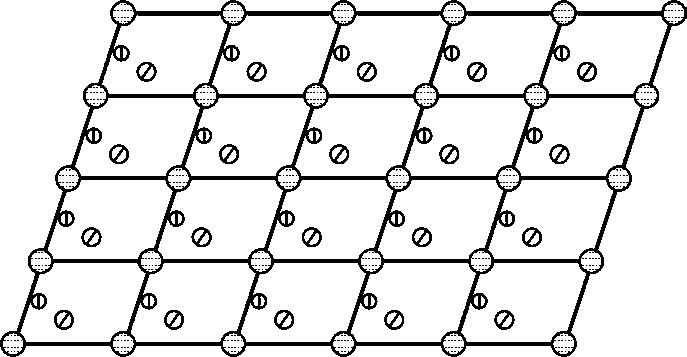
\includegraphics[width=0.5\linewidth]{crystall_lattice.png}}
\caption{Кристаллическая решетка с базисом, состоящим из трех атомов}
\label{pic:crystall_lattice}
\end{figure}
Группу атомов, относящуюся к данному узлу, называют базисом. В оббщем случае 
узел кристаллической решетки не обязательно совмещать с каким-либо 
атомом, но обычно это делают из соображений удобства. Различают 
простые решетки, базис которых состоит из одного атома, и сложные, 
к каждому узлу которых относятся два или более атомов~\cite{Vladimirov_book}.


Основным свойством кристаллической решетки является наличие 
трансляционной симметрии. Для двумерной решетки это значит, что она 
совмещается сама с собой при перемещении на вектор трансляции решетки:
\begin{equation}
	\label{translation_vector}
	\vec{t}_{hk}=h\cdot\vec{t}_x+k\cdot\vec{t}_y
\end{equation}
где $\vec{t}_x$ и $\vec{t}_y$ - основные вектора трансляции, а 
\textit{h} и \textit{k} - любые целые числа. Обычно в качестве основных
векторов выбирают наименьшие по длине. Так, в случае решетки, изображенной на рис~\ref{pic:crystall_lattice2}, отдают предпочтение 
\begin{figure}[!ht]
\center{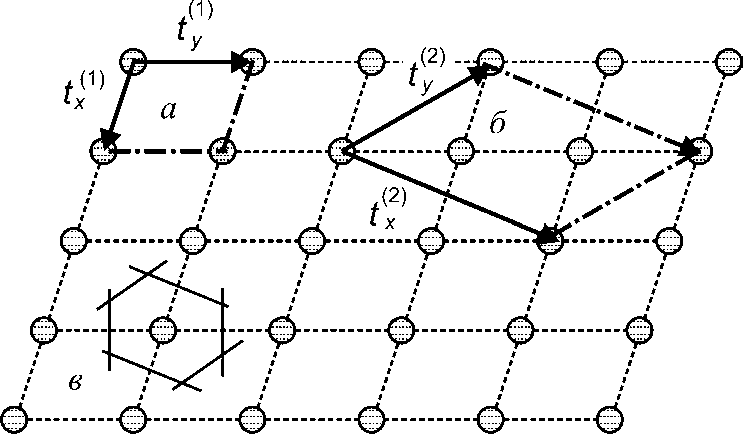
\includegraphics[width=0.5\linewidth]{crystall_lattice2.png}}
\caption{Возможные варианты выбора основных векторов трансляции и элементарной ячейки. а - примитивная ячейка; б - элементарная ячейка;
в - ячейка Вигнера-Зейтца}
\label{pic:crystall_lattice2}
\end{figure}
вектору $\vec{t}^{(1)}_x$ перед $\vec{t}^{(2)}_x$.


Элемент решетки, трансляцией которого на различные вектора $\vec{t}_{hk}$
может быть получена вся решетка целиком, называют элементарной ячейкой.
Частным случаем элементарной ячейки является примитивная, имеющая минимальную из всех возможных площадь.


Другой способ конструирования примитивной ячейки заключается в выделении
такой области решетки, все точки которой расположены ближе к фиксированному узлу (центр ячейки), чем к любому другому. Такую ячейку
называют ячейкой Вигнера-Зейтца рис.~\ref{pic:crystall_lattice2}в.


Кроме трансляционной симметрии двухмерные решетки могут обладать
некоторым числом операций точечной и осевой симметрии. По симметрии
все кристаллические решетки, их еще называют решетками Браве, можно
разделить на 5 типов:
\begin{itemize}
	\item Косоугольная решетка с произвольным соотношением длин основных векторов~\ref{pic:2d_lattices}a;
	\item Прямоугольная, инвариантна относительно плоскости зеркального отражения~\ref{pic:2d_lattices}б;
	\item Прямоугольная центрированная, имеет базис из двух или более атомов~\ref{pic:2d_lattices}в;
	\item Квадратная решетка, имеет ось четвертого порядка~\ref{pic:2d_lattices}г;
	\item Гексагональная решетка, инвариантна к повороту на $2\pi/6$~\ref{pic:2d_lattices}д;
\end{itemize}
\begin{figure}[!ht]
\center{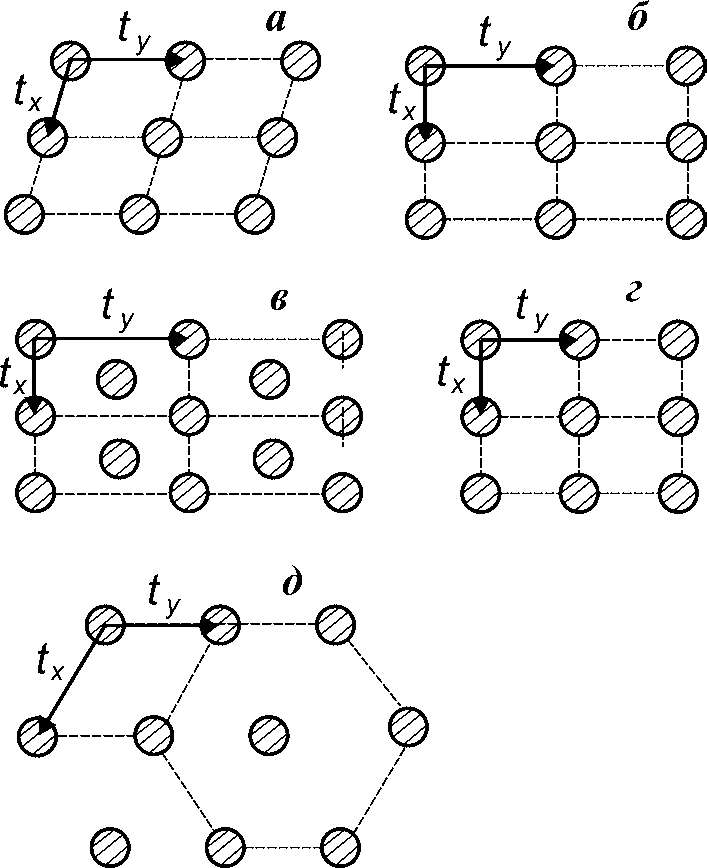
\includegraphics[width=0.4\linewidth]{2d_lattices.png}}
\caption{Типы двумерных решеток: a - косоугольная; б - прямоугольная;
в - прямоугольная центрированная; г - квадратная; д - гексагональная}
\label{pic:2d_lattices}
\end{figure}


Поверхности монокристаллов принято обозначать индексами Миллера,
соответствующими плоскости, параллельной поверхности. В случае 
плотноупакованных граней этого вполне достаточно, чтобы представить себе
расположение атомов, если оно не отличается от имеющегося в объеме. На 
рис.~\ref{pic:atoms_in_lattice} приведено расположение атомов для
некоторых кристаллических структур. Например, достаточно очевидно 
расположение атомов на грани(100) кристалла, имеющего гранецентрированную
кубическую структуру: элементарная ячейка имеет квадратную форму. Если
смотреть сверху, то видны атомы второго слоя. В случае грани(111) 
имеется гексагональная упаковка, что обеспечивает максимальную 
плотность атомов, причем сверху просматриваются не только атомы следующего слоя, но и третьего~\cite{Vladimirov_book}.
\begin{figure}[!ht]
\center{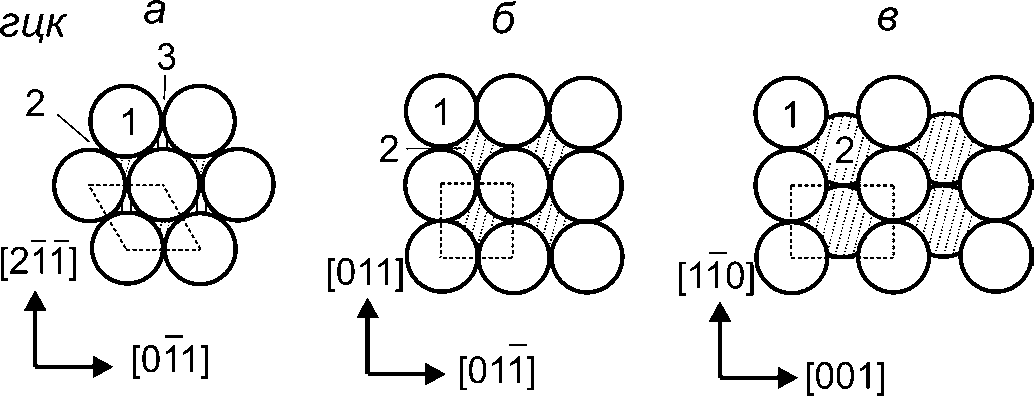
\includegraphics[width=0.6\linewidth]{atoms_in_lattice.png}}
\caption{Расположение атомов на плотноупакованных гранях кристаллов,
имеющих гранецентрированную кубическую структуру(гцк), вид сверху:
а-(111); б-(100); в-(110); 1-атомы первого слоя; 2-второго; 3-третьего.}
\label{pic:atoms_in_lattice}
\end{figure}





\subsection{Электронная структура кристаллов и кристаллических поверхностей} \label{sect1_1_2}
Для описания электронной структуры кристаллов или кристаллических 
поверхностей, обладающих пространственной периодичностью используется
зонная модель~\cite{Kittel1976}. В общем случае задача об электронах 
твердого тела является многоэлектронной задачей, потому что полный 
гамильтониан в твердых телах содержит не только одноэлектронные 
потенциалы, описывающие взаимодействие легкого электрона с массивным 
ядром, но и потенциалы взаимодействия электронов между собой~\cite{Simonov_disser}.
В приближении свободных электронов такое взаимодействие описывается
с помощью эффективного одноэлектронного потенциала $U(\vec{r})$. 
Вне зависимости от формы этого потенциала, для идеального периодического
кристалла он будет удовлетворять условию периодичности:
\begin{equation}
	\label{one_electron_potential}
	U(\vec{r})=U(\vec{r}+\vec{R})
\end{equation}
для всех векторов $\vec{R}$, принадлежащих решетке Браве.


В рамках одноэлектронной модели движение электрона в кристалле описывается
уравнением Шредингера:
\begin{equation}
	\label{Shredinger_equation}
	H\psi=\left(\frac{-\hbar^2}{2m}\Delta+U(\vec{r})\right)\psi=\varepsilon\psi
\end{equation}
где $U(\vec{r})$ - эффективный потенциал, удовлетворяющий условию~\ref{one_electron_potential}.


Следствием периодичности потенциала является очень важное свойство 
стационарных состояний - теорема Блоха. Согласно этой теореме 
собственные состояния оператора \textit{H} можно выбрать таким образом,
чтобы с каждым из них был связан некоторый волновой вектор $\vec{k}$ и 
для любого $\vec{R}$ в решетке Браве выполнялось равенство:
\begin{equation}
	\label{equaliation_of_wave_func}
	\psi(\vec{r}+\vec{R})=e^{i\vec{k}\vec{R}}\psi(\vec{r})
\end{equation}


При этом $\psi(\vec{r})$ представима в виде Блоховской волны:
\begin{equation}
	\label{Bloh_wave}
	\psi(\vec{r})=e^{i\vec{k}\vec{R}}u(\vec{r})
\end{equation}
где
\begin{equation}
	\label{u_wave}
	u(\vec{r}+\vec{R})=u(\vec{r})
\end{equation}


Введенный вектор $\vec{k}$ является квантовым числом, которое 
характеризует трансляционную симметрию периодического потенциала. 
В общей задаче о движении в периодическом потенциале он играет ту же роль, что и волновой вектор $\vec{k}$ свободного электрона в теории 
Зоммерфельда~\cite{Kittel1976}. Однако, нужно заметить, что в отличие 
от состояний свободного электрона, в периодическом потенциале одно
и то же состояние электрона характеризуется бесконечным набором векторов
$\vec{k}, \vec{k'}, \vec{k''}$ и т. д., отличающихся друг от друга на вектор $\vec{K}$ обратной решетки (см.~\ref{equaliation_of_wave_func}).
По этой причине вектор $\vec{k}$ называют квазиволновым вектором, а
$\hbar\vec{k}$ - соответствующим квазиимпульсом. Так как для двух
значений $\vec{k}$, отличающихся друг от друга на вектор обратной 
решетки, все волновые функции и энергетические уровни совпадают,
для полного описания всей совокупности уровней достаточно ограничить
область значений $\vec{k}$ одной элементарной ячейкой.
Зоной Бриллюэна называют область обратного пространства, которое включает
в себя все множество неэквивалентных значений квазиволнового вектора.
Для обратной решетки первая зона Бриллюэна совпадает с ячейкой 
Вигнера-Зейтца~\cite{Kittel1976}. По теореме Блоха можно показать, что 
энергетические уровни электрона в периодическом потенциале могут быть описаны с помощью непрерывных функций $\varepsilon_n(\vec{k})$(\textit{n} - 
номер энергетической зоны), каждая из которых имеет периодичность
обратной решетки. Структуру твердого тела определяют именно эти 
функции\cite{Simonov_disser}.
\begin{figure}[!ht]
\center{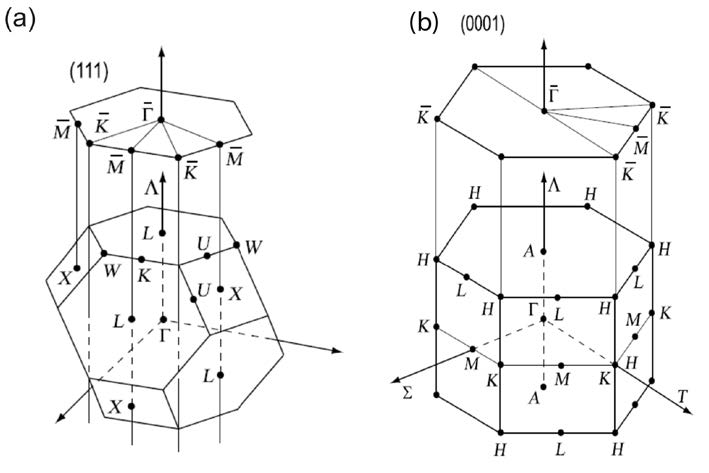
\includegraphics[width=0.7\linewidth]{zones.png}}
\caption{Связь между двумерной зоной Бриллюэна плоскости(111) fcc
кристалла (a), плоскости (0001) гексагонального кристалла (b) и 
объемной зоной Бриллюэна~\cite{Hufner2019}}
\label{pic:Brilluen_zones}
\end{figure}


Для анализа систем с пространственной периодичностью концепция
зон Бриллюэна играет очень важную роль. На рис.~\ref{pic:Brilluen_zones}
показаны двумерные зоны Бриллюэна для плотноупакованной грани (111) 
гранецентрированного кубического (fcc) кристалла и грани (0001)
гексагонального кристалла. Так же на этом рисунке показана их связь с 
объемными Зонами Бриллюэна~\cite{Hufner2019}. 





\section{Низкоразмерные структуры} \label{sect1_2}

\section{Гексагональный нитрид бора} \label{sect1_3}
